
%(BEGIN_QUESTION)
% Copyright 2015, Tony R. Kuphaldt, released under the Creative Commons Attribution License (v 1.0)
% This means you may do almost anything with this work of mine, so long as you give me proper credit

The following graph shows the signal strength received by a guided-wave radar (GWR) level instrument over time:

$$\includegraphics[width=15.5cm]{i00289x01.eps}$$

Explain how the graph will change if:

\begin{itemize}
\item{} The liquid level increases
\item{} The dielectric constant ($\epsilon$) of the liquid decreases
\item{} The density of the liquid decreases (assuming constant $\epsilon$)
\item{} A liquid-liquid interface consisting of two liquids with different densities is introduced into the vessel
\end{itemize}

Also, explain what {\it UNZ} refers to (the {\it Upper Null Zone}).

\vskip 20pt \vbox{\hrule \hbox{\strut \vrule{} {\bf Suggestions for Socratic discussion} \vrule} \hrule}

\begin{itemize}
\item{} Describe a practical reason for configuring a radar transmitter to have an upper null zone, and how this differs from a radar instrument's {\it transition zones}.
\item{} Explain why the timing of {\it both} the echo pulse and the end-of-probe pulse will shift as liquid level changes in this system.
\end{itemize}

\underbar{file i00289}
%(END_QUESTION)





%(BEGIN_ANSWER)

%(END_ANSWER)





%(BEGIN_NOTES)

If the liquid level were to increase, the echo pulse would happen sooner (closer to the reference pulse).

\vskip 10pt

If the liquid's permittivity were to decrease, the end-of-probe pulse would happen sooner because the velocity of propagation through the liquid would increase.  However, the echo pulse would remain fixed in position because the gas's propagation velocity would remain fixed.  The echo pulse would be less strong, though, owing to a decreased power reflection factor.

\vskip 10pt

If the liquid's density were to decrease with no change in permittivity, the echo timing would not change at all.  This illustrates the advantageous behavior of radar level instruments with regard to liquid density.

\vskip 10pt

If a liquid-liquid interface were to be introduced into the vessel, the graph would exhibit an additional echo pulse, like this:

$$\includegraphics[width=15.5cm]{i00289x03.eps}$$

\vskip 10pt

The Upper Null Zone is a range programmed in to the digital radar instrument where the instrument will ignore any reflected signals.

\vskip 30pt

\filbreak

An advanced concept to consider is that if the liquid level were to increase, the echo pulse would move closer to the reference pulse in time, but the end-of-probe pulse would also move further away from the reference pulse, like this:

$$\includegraphics[width=15.5cm]{i00289x02.eps}$$

The reason the end-of-probe pulse does not maintain a fixed position in time is due to the fact that the speed of light in liquid is slower than the speed of light in a vapor.  This effect naturally follows the change in permittivity from vapor to liquid:

$$v = {c \over \sqrt{\epsilon_r}}$$

Therefore, a greater liquid level means a shorter vapor path and thus a shorter time to receive the echo pulse.  However, it also means a longer echo path for the signal through liquid, with a slower speed of propagation, which means the time for the end-of-probe echo pulse to return to the instrument will be greater than the change in time for the first echo pulse.

%INDEX% Measurement, level: radar

%(END_NOTES)


